\documentclass[11pt, oneside]{article}   	% use "amsart" instead of "article" for AMSLaTeX format
\usepackage[margin = 1in]{geometry}                		% See geometry.pdf to learn the layout options. There are lots.
\geometry{letterpaper}                   		% ... or a4paper or a5paper or ... 
%\geometry{landscape}                		% Activate for rotated page geometry
\usepackage[parfill]{parskip}    		% Activate to begin paragraphs with an empty line rather than an indent
\usepackage{graphicx, ulem, tikz, multicol, tabularx}				% Use pdf, png, jpg, or eps§ with pdflatex; use eps in DVI mode
								% TeX will automatically convert eps --> pdf in pdflatex		
\usepackage{amssymb, enumerate}

%SetFonts

%SetFonts


\title{Math F113X: Homework Set 5}
%\author{The Author}
\date{}							% Activate to display a given date or no date

\begin{document}
\maketitle
%\section{}
%\subsection{}

%Homework assignment 1 is:
%\vspace{-1.5cm}


\fbox{\parbox{\textwidth}{

Answer the following problems from the Graph Theory section \emph{in the order assigned.}
\begin{quote} A, B, 2, 23, C, D \end{quote}
}}

\quad\\

\textbf{Problem A:} Use the drawing of Graph G (in box) to answer the questions. \\

\fbox{
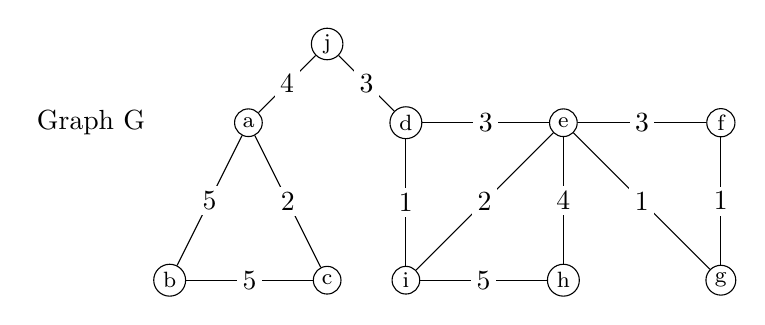
\begin{tikzpicture}[scale=1]
\node at (-1,2){Graph G};
\tikzstyle{vtx}=[circle, draw, fill=black!0,
                        inner sep=1.5pt, minimum width=10pt, font = \footnotesize]
 \tikzstyle{lbl}=[midway, inner sep = 2 pt, fill = white]                   
\node[vtx](a) at (1,2){a};
\node[vtx](b) at (0,0){b};
\node[vtx](c) at (2,0){c};
\node[vtx](d) at (3,2){d};
\node[vtx](e) at (5,2){e};
\node[vtx](f) at (7,2){f};
\node[vtx](g) at (7,0){g};
\node[vtx](h) at (5,0){h};
\node[vtx](i) at (3,0){i};
\node[vtx](j) at (2,3){j};
\foreach \i/\j/\k in {a/b/5,a/c/2,b/c/5,a/j/4,d/j/3,d/i/1,d/e/3, e/i/2,i/h/5,e/h/4,e/f/3,e/g/1,f/g/1}{\draw (\i) -- node[lbl]{\k} (\j);}
\end{tikzpicture}
}
\begin{enumerate}
\item Draw two different spanning trees of Graph G.
\item Determine the total weight of each tree from part 1 above. 
\item Find a minimum weight spanning tree. (Use any method you like, including guess-and-check.)
\end{enumerate}

\quad \\

\textbf{Problem B:} Use Kruskal's Algorithm to find a minimum cost
spanning tree in each graph below. Make sure to show appropriate
work. A good way to do this is to make a table like the one
below. List every edge in \emph{ascending order of weight} (that is, smallest to largest) in the first
column. List the corresponding weight in the second column. In the
third column, use a checkmark to indicate that you are using the edge
in your spanning tree and an ``x'' to indicate that you are not.\\
%\begin{multicols}{2}
\begin{tabularx}{\textwidth}{X X}

\fbox{
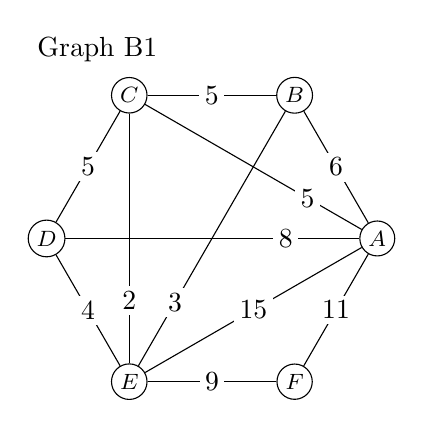
\begin{tikzpicture}[scale=0.7, baseline=(current bounding box.north)]
\tikzstyle{vtx}=[circle, draw, fill=black!0,
                        inner sep=1.5pt, minimum width=10pt, font = \footnotesize]
 \tikzstyle{lbl}=[midway, inner sep = 2 pt, fill = white] 
 \tikzstyle{lbb}=[pos=0.25, inner sep = 2 pt, fill = white]
	\node[vtx] (A) at (0:3){$A$};
	\node[vtx] (B) at (60:3){$B$};
	\node[vtx] (C) at (120:3){$C$};
	\node[vtx] (D) at (180:3){$D$};
	\node[vtx] (E) at (240:3){$E$};
	\node[vtx] (F) at (300:3){$F$};
	
\foreach \i/\j/\k in {A/B/6,A/E/15,B/C/5,C/D/5,D/E/4,E/F/9,A/F/11}{\draw (\i) -- node[lbl]{\k} (\j);}
\foreach \i/\j/\k in {E/C/2,A/D/8,A/C/5,E/B/3}{\draw (\i) -- node[lbb]{\k} (\j);}

\node[anchor=south west, yshift=2pt] at (current bounding box.north west) {Graph B1};
\end{tikzpicture}
}

& 
\vspace{0pt}
\begin{tabular}{c|c|c}
edge & weight & used? \\
\hline
 &  & \\
 &  & \\
 &  & \\
 &  & \\
 &  & \\
 &  & \\
 &  & \\
 &  & \\
 &  & \\
 &  & \\
 &  & \\
\end{tabular}

\\


%Graph $B_2$\\
\fbox{
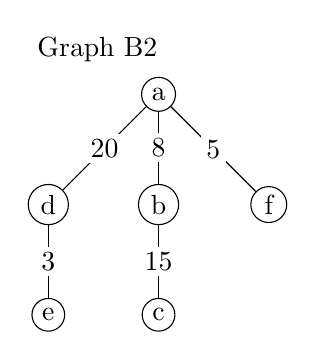
\begin{tikzpicture}[scale=0.7,  baseline=(current bounding box.north)]
\node[draw,circle, inner sep=2pt](a) at (0,4){a};
\node[draw,circle, inner sep=2pt](b) at (0,2){b};
\node[draw,circle, inner sep=2pt](d) at (-2,2){d};
\node[draw,circle, inner sep=2pt](f) at (2,2){f};
\node[draw,circle, inner sep=2pt](c) at (0,0){c};
\node[draw,circle, inner sep=2pt](e) at (-2,0){e};
 \tikzstyle{lbl}=[midway, inner sep = 2 pt, fill = white]
 \foreach \i/\j/\k in {a/d/20,a/b/8,a/f/5,d/e/3,b/c/15}{\draw (\i) -- node[lbl]{\k} (\j);}
 \node[anchor=south west, yshift=2pt] at (current bounding box.north west) {Graph B2};

\end{tikzpicture}
}

& 
\vspace{0pt}
\begin{tabular}{c|c|c}
edge & weight & used? \\
\hline
 &  & \\
 &  & \\
 &  & \\
 &  & \\
 &  & \\
 &  & \\
 &  & \\
 &  & \\
 &  & \\
 &  & \\
 &  & \\
\end{tabular}
\end{tabularx}

\hrulefill

\textbf{Problem C:} Describe one real-world situation in which it would be useful to find
a minimal spanning tree for a graph. Be sure to clearly describe the
overall scenario, specify what the vertices represent, specify what
the edges represent, specify what the edge weights represent, and
state why you would want to find a minimal weight spanning tree.


\hrulefill

\textbf{Problem D:} For each graph below, (i) determine if it has an Euler circuit and (ii) determine if it has an Euler path. Justify your answer. \\

\begin{multicols}{3}
Graph $C_1$\\
\fbox{
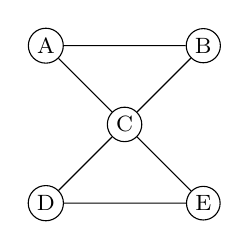
\begin{tikzpicture}
\tikzstyle{vtx}=[circle, draw, fill=black!0,
                        inner sep=1.5pt, minimum width=10pt, font = \footnotesize]
	\node[vtx] (A) at (-1,1){A};
	\node[vtx] (B) at (1,1){B};
	\node[vtx] (C) at (0,0){C};
	\node[vtx] (D) at (-1,-1){D};
	\node[vtx] (E) at (1,-1){E};
\draw (A)--(B)--(C)--(D)--(E)--(C)--(A);
\end{tikzpicture}
}

\columnbreak

Graph $C_2$\\
\fbox{
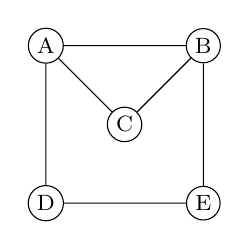
\begin{tikzpicture}
\tikzstyle{vtx}=[circle, draw, fill=black!0,
                        inner sep=1.5pt, minimum width=10pt, font = \footnotesize]
	\node[vtx] (A) at (-1,1){A};
	\node[vtx] (B) at (1,1){B};
	\node[vtx] (C) at (0,0){C};
	\node[vtx] (D) at (-1,-1){D};
	\node[vtx] (E) at (1,-1){E};
\draw (A)--(B)--(C)(B)--(E)--(D)--(A)--(C);
\end{tikzpicture}
}
\columnbreak

Graph $C_3$\\
\fbox{
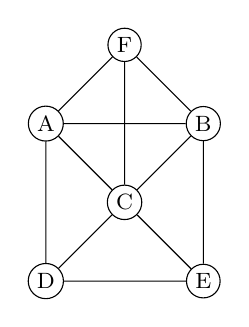
\begin{tikzpicture}
\tikzstyle{vtx}=[circle, draw, fill=black!0,
                        inner sep=1.5pt, minimum width=10pt, font = \footnotesize]
	\node[vtx] (A) at (-1,1){A};
	\node[vtx] (B) at (1,1){B};
	\node[vtx] (C) at (0,0){C};
	\node[vtx] (D) at (-1,-1){D};
	\node[vtx] (E) at (1,-1){E};
	\node[vtx] (f) at (0,2){F};
\draw (A)--(B)--(C)--(D)--(E)--(C)--(A)--(D)(E)--(B);
\draw (A)--(f)--(B)(C)--(f);
\end{tikzpicture}
}
\end{multicols}

\hrulefill

Remember to write up your homework solutions according to the homework writeup guidelines. 

Homework is graded using the following rubric for each problem (or problem part):

\begin{description}
\item[2 points:] You provided a complete answer, with supporting work, written up clearly
\item[1 point:] Some attempt at a solution, but incomplete writeup / unclear / illegible / no answer
\item[1 point:] Only an answer, with no supporting work 
\item[0 points:] Missing.
\end{description}

After you do the homework, you need to check your answers against the solutions! Then figure out your errors (if any) and revise your homework before you submit it. 

\end{document}  
%%% Local Variables:
%%% mode: LaTeX
%%% TeX-master: t
%%% End:
